
\documentclass[a4paper]{article}

\usepackage[english]{babel}
\usepackage[utf8]{inputenc}
\usepackage{amsmath}
\usepackage{graphicx}
\usepackage[colorinlistoftodos]{todonotes}
\usepackage{float}
\usepackage{hyperref}
\setlength\parindent{0pt}

\title{Footpath Planning for Example-driven Procedural Road Networks}

\author{Alexander Hjelm}

\date{\today}

\begin{document}
\maketitle

\section{Abstract}

\begin{figure}[H]
\centering
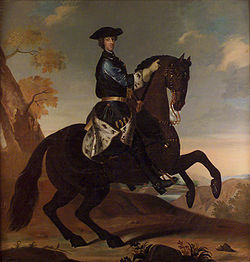
\includegraphics[height=0.5\textheight]{test_image}
\caption{En typisk rymdhiss enligt Wikipedia. Bildkälla (\cite{sampleitem1}).}
\label{fig:space}
\end{figure}

This report covers... \cite{sampleitem2}

\begin{thebibliography}{9}
\bibitem{sampleitem1}
Title 1, \\ 
\href{https://en.wikipedia.org/wiki/Geostationary\_ orbit}{https://en.wikipedia.org/wiki/Geostationary\_ orbit}.

\bibitem{sampleitem2}
Title 2, \\ 
\href{https://sv.wikipedia.org/wiki/SpaceX}{https://sv.wikipedia.org/wiki/SpaceX}.

\end{thebibliography}


\end{document}
